\documentclass[12pt,a4paper]{article}
\usepackage[utf8]{inputenc}
\usepackage[T1]{fontenc}
\usepackage{lmodern}
\usepackage{graphicx}
\usepackage{hyperref}
\usepackage{listings}
\usepackage{xcolor}
\usepackage{geometry}
\usepackage[polish]{babel}
\usepackage{tikz}
\usetikzlibrary{shapes.geometric, arrows, positioning, fit, arrows.meta}

\geometry{a4paper, margin=2.5cm}

% Code listing settings
\definecolor{codebackground}{rgb}{0.95,0.95,0.95}
\definecolor{codekeyword}{rgb}{0.08,0.39,0.63}
\definecolor{codecomment}{rgb}{0.13,0.55,0.13}
\definecolor{codestring}{rgb}{0.7,0.14,0.14}

\lstset{
  basicstyle=\ttfamily\small,
  keywordstyle=\color{codekeyword}\bfseries,
  stringstyle=\color{codestring},
  commentstyle=\color{codecomment},
  backgroundcolor=\color{codebackground},
  breakatwhitespace=false,
  breaklines=true,
  captionpos=b,
  keepspaces=true,
  showspaces=false,
  showstringspaces=false,
  showtabs=false,
  tabsize=2,
  frame=single,
  frameround=tttt,
  framesep=5pt,
  xleftmargin=10pt,
  xrightmargin=10pt
}

% Kotlin language definition for listings
\lstdefinelanguage{Kotlin}{
  keywords={package, import, class, interface, object, val, var, fun, for, while, if, else, when, try, catch, finally, return, break, continue, companion, data, suspend},
  sensitive=true,
  morecomment=[l]{//},
  morecomment=[s]{/*}{*/},
  morestring=[b]",
  morestring=[s]{"""}{"""}
}

% JSON language definition for listings
\lstdefinelanguage{json}{
  basicstyle=\normalfont\ttfamily,
  commentstyle=\color{codecomment},
  stringstyle=\color{codestring},
  keywordstyle=\color{codekeyword},
  numbers=left,
  numberstyle=\scriptsize,
  stepnumber=1,
  numbersep=8pt,
  showstringspaces=false,
  breaklines=true,
  literate=
     *{0}{{{\color{codekeyword}0}}}{1}
      {1}{{{\color{codekeyword}1}}}{1}
      {2}{{{\color{codekeyword}2}}}{1}
      {3}{{{\color{codekeyword}3}}}{1}
      {4}{{{\color{codekeyword}4}}}{1}
      {5}{{{\color{codekeyword}5}}}{1}
      {6}{{{\color{codekeyword}6}}}{1}
      {7}{{{\color{codekeyword}7}}}{1}
      {8}{{{\color{codekeyword}8}}}{1}
      {9}{{{\color{codekeyword}9}}}{1}
      {:}{{{\color{codecomment}{:}}}}{1}
      {,}{{{\color{codecomment}{,}}}}{1}
      {\{}{{{\color{codekeyword}{\{}}}}{1}
      {\}}{{{\color{codekeyword}{\}}}}}{1}
      {[}{{{\color{codekeyword}{[}}}}{1}
      {]}{{{\color{codekeyword}{]}}}}{1},
}

\title{\textbf{JSONPlaceholder pobieranie postów}\\
\large Dokumentacja techniczna}
\author{Maciej Kasik}
\date{\today}

\begin{document}

\maketitle
\tableofcontents
\newpage

\section{Opis projektu}

\subsection{Cel i zakres}
Aplikacja służy do pobierania postów z serwisu JSONPlaceholder API i zapisywania ich w postaci indywidualnych plików JSON. Każdy post jest zapisywany w oddzielnym pliku o nazwie odpowiadającej identyfikatorowi posta.

Aplikacja obsługuje trzy środowiska pracy:
\begin{itemize}
    \item \textbf{Development} -- środowisko deweloperskie do pracy lokalnej
    \item \textbf{Staging} -- środowisko testowe
    \item \textbf{Production} -- środowisko produkcyjne
\end{itemize}

\subsection{Technologie}
\begin{itemize}
    \item Kotlin 1.9.0 - język programowania
    \item Retrofit 2.9.0 - komunikacja HTTP
    \item OkHttp 4.10.0 - klient HTTP
    \item Gson 2.10.1 - obsługa formatu JSON
    \item Coroutines 1.7.3 - programowanie asynchroniczne
    \item Gradle - system budowania
\end{itemize}

\subsection{Wymagania systemowe}
\begin{itemize}
    \item JDK 8+
    \item Dostęp do internetu
\end{itemize}

\section{Wymagania projektowe}

\subsection{Wymagania funkcjonalne}
Poniższe wymagania funkcjonalne określają, co system musi robić, aby zaspokoić potrzeby użytkownika:

\begin{enumerate}
    \item \textbf{Pobieranie danych} -- System musi pobierać kompletną listę postów z API JSONPlaceholder poprzez wywołanie endpointu \texttt{/posts}.
    
    \item \textbf{Zapisywanie plików} -- Każdy pobrany post musi zostać zapisany jako osobny plik w formacie JSON.
    
    \item \textbf{Identyfikacja plików} -- Nazwy plików wyjściowych muszą odpowiadać identyfikatorom postów (np. \texttt{1.json}, \texttt{2.json}).
    
    \item \textbf{Katalog docelowy} -- System musi automatycznie tworzyć katalog docelowy, jeśli ten nie istnieje w momencie uruchomienia aplikacji.
    
    \item \textbf{Raportowanie} -- System musi raportować postęp operacji w konsoli, w tym:
    \begin{itemize}
        \item liczbę pobranych postów
        \item liczbę pomyślnie zapisanych plików
        \item podsumowanie całej operacji
    \end{itemize}
    
    \item \textbf{Obsługa błędów} -- System musi wykrywać i informować o błędach występujących podczas:
    \begin{itemize}
        \item komunikacji z API
        \item przetwarzania danych
        \item operacji zapisu na dysku
    \end{itemize}
\end{enumerate}

\subsection{Wymagania niefunkcjonalne}
Poniższe wymagania niefunkcjonalne określają, jak system ma działać i jakie aspekty jakościowe powinien spełniać:

\begin{enumerate}
    \item \textbf{Wydajność} -- System musi wykorzystywać asynchroniczne mechanizmy komunikacji sieciowej, aby zminimalizować czas oczekiwania na odpowiedź API.
    
    \item \textbf{Niezawodność} -- System musi obsługiwać sytuacje wyjątkowe, takie jak:
    \begin{itemize}
        \item brak dostępu do sieci
        \item niedostępność usługi API
        \item brak uprawnień do zapisu na dysku
    \end{itemize}
    
    \item \textbf{Modularność} -- Kod systemu musi być zorganizowany w logiczne komponenty o jednorodnych odpowiedzialnościach, zgodnie z zasadami Clean Architecture.
    
    \item \textbf{Rozszerzalność} -- System musi umożliwiać łatwe rozszerzenie o dodatkowe funkcjonalności, takie jak:
    \begin{itemize}
        \item obsługa innych endpointów JSONPlaceholder API
        \item konfigurację parametrów pracy (np. wybór katalogu docelowego)
        \item filtry danych
    \end{itemize}
    
    \item \textbf{Bezpieczeństwo} -- System musi wykonywać bezpieczne operacje wejścia/wyjścia, unikając typowych błędów, takich jak race conditions czy wycieki zasobów.
    
    \item \textbf{Utrzymywalność} -- Kod źródłowy musi być dokumentowany zgodnie ze standardami, a architektura musi ułatwiać jego późniejsze modyfikacje.
\end{enumerate}

\section{Architektura systemu}

\subsection{Diagramy UML}

W celu lepszego zobrazowania architektury systemu, poniżej przedstawiono diagramy UML: diagram klas, diagram sekwencji oraz diagram komponentów.

\subsubsection{Diagram klas}

Diagram klas przedstawia strukturę statyczną systemu, pokazując klasy, ich atrybuty, metody oraz relacje między nimi.

\begin{figure}[h]
\centering
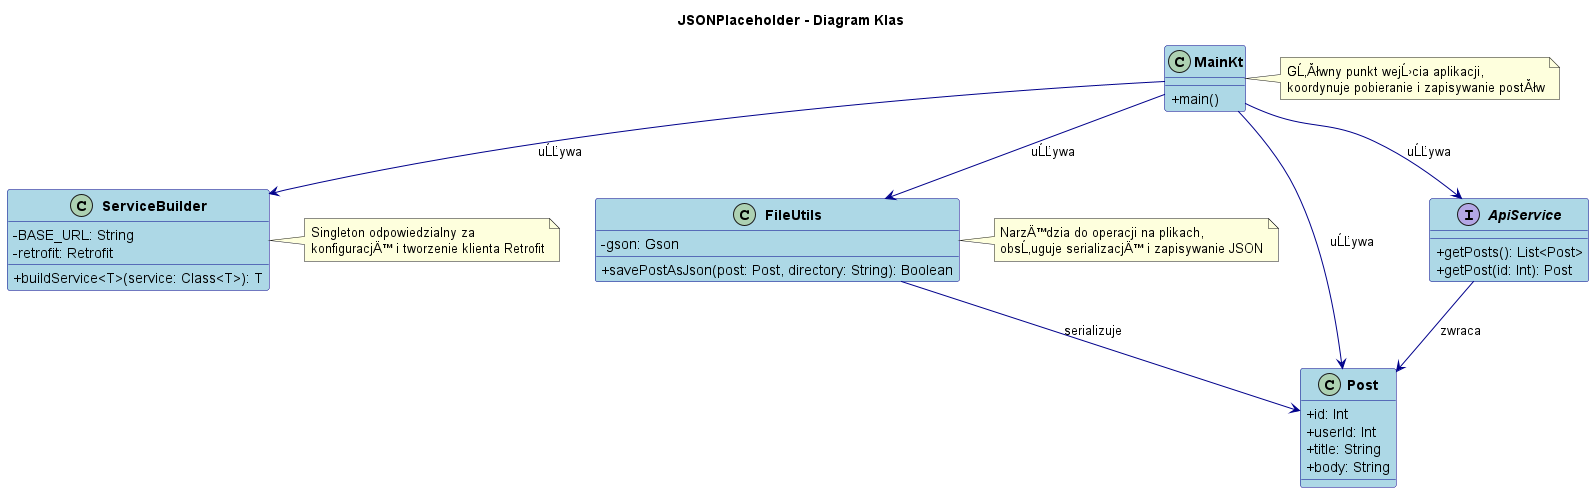
\includegraphics[width=0.9\textwidth]{plantuml/class_diagram.png}
\caption{Diagram klas systemu pobierania postów}
\label{fig:class-diagram}
\end{figure}

\subsubsection{Diagram sekwencji}

Diagram sekwencji ilustruje interakcje między komponentami systemu w czasie, pokazując przepływ komunikacji podczas pobierania i zapisywania postów.

\begin{figure}[h]
\centering
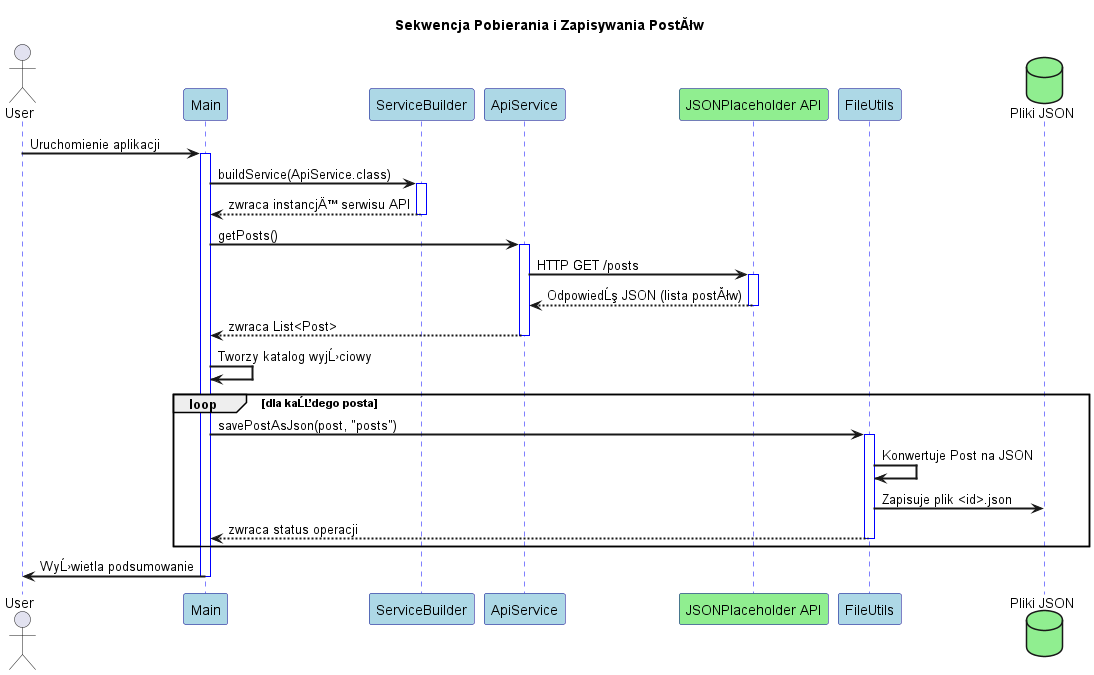
\includegraphics[width=0.9\textwidth]{plantuml/sequence_diagram.png}
\caption{Diagram sekwencji pobierania i zapisywania postów}
\label{fig:sequence-diagram}
\end{figure}

\subsubsection{Diagram komponentów}

Diagram komponentów przedstawia komponenty systemu oraz ich wzajemne zależności, ukazując ogólną strukturę aplikacji.

\begin{figure}[h]
\centering
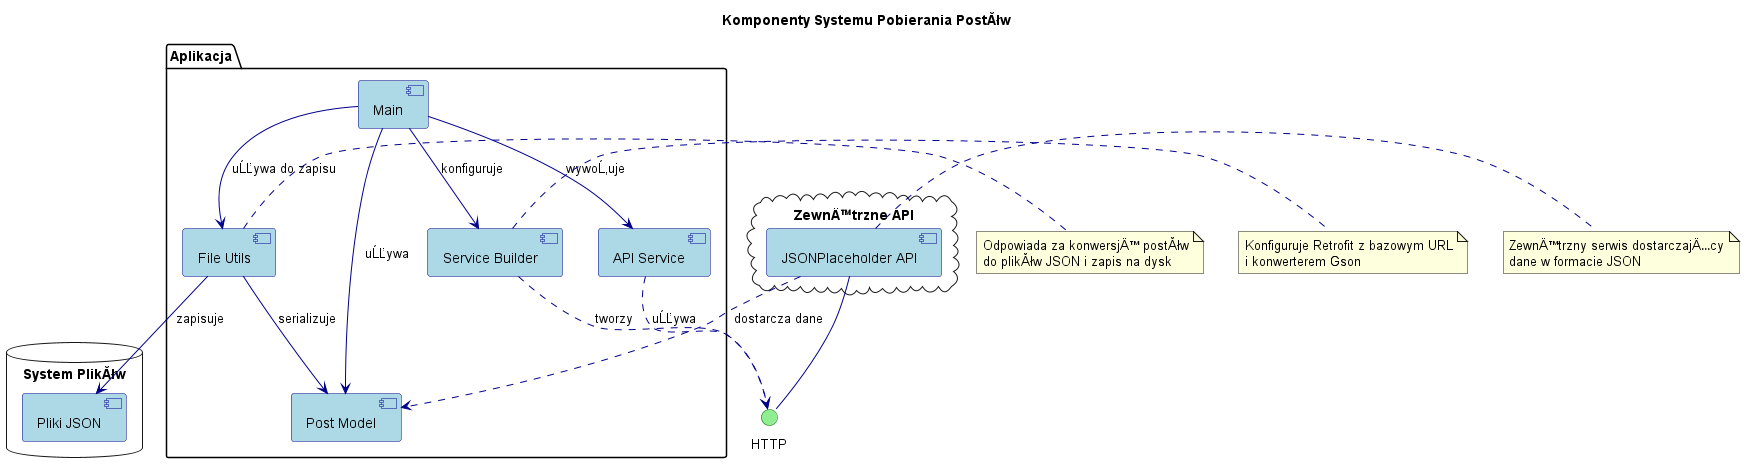
\includegraphics[width=0.9\textwidth]{plantuml/component_diagram.png}
\caption{Diagram komponentów systemu}
\label{fig:component-diagram}
\end{figure}

\subsection{Opis komponentów}

\begin{itemize}
    \item \textbf{Model Post} - klasa danych reprezentująca strukturę posta: id, userId, title, body
    
    \item \textbf{Serwis API} - interfejs definiujący endpointy API:
    \begin{itemize}
        \item \texttt{getPosts()} - pobieranie listy wszystkich postów
        \item \texttt{getPost(id)} - pobieranie pojedynczego posta
    \end{itemize}
    
    \item \textbf{Konstruktor Serwisu} - fabryka klientów REST:
    \begin{itemize}
        \item Konfiguracja bazowego URL dla aktualnego środowiska
        \item Konfiguracja konwertera JSON (Gson)
        \item Konfiguracja klienta HTTP z parametrami zależnymi od środowiska
        \item Włączanie/wyłączanie logowania na podstawie konfiguracji środowiskowej
    \end{itemize}
    
    \item \textbf{Narzędzia Plikowe} - operacje na plikach:
    \begin{itemize}
        \item Serializacja obiektów do formatu JSON
        \item Tworzenie katalogów
        \item Zapisywanie danych do plików
        \item Czyszczenie katalogów wyjściowych (w trybie development)
    \end{itemize}
    
    \item \textbf{Główna Aplikacja} - przepływ logiki biznesowej:
    \begin{itemize}
        \item Przetwarzanie parametrów wywołania
        \item Wybór środowiska uruchomieniowego
        \item Pobieranie postów z API
        \item Koordynacja przetwarzania danych
        \item Zapisywanie do plików
    \end{itemize}
    
    \item \textbf{Konfiguracja Środowiskowa} - zarządzanie konfiguracją:
    \begin{itemize}
        \item Określenie parametrów dla różnych środowisk
        \item Wybór konfiguracji na podstawie parametrów lub zmiennych środowiskowych
        \item Dostarczanie ustawień dla pozostałych komponentów
    \end{itemize}
\end{itemize}

\section{Przepływ danych}

\subsection{Pobieranie danych}
\begin{enumerate}
    \item Utworzenie instancji serwisu API za pomocą konstruktora serwisu
    \item Wysłanie asynchronicznego żądania HTTP GET do \texttt{/posts}
    \item Deserializacja odpowiedzi JSON do listy obiektów Post
\end{enumerate}

\subsection{Przetwarzanie i zapisywanie}
\begin{enumerate}
    \item Utworzenie katalogu wyjściowego \texttt{posts} (jeśli nie istnieje)
    \item Iteracja przez listę pobranych postów
    \item Dla każdego posta:
    \begin{itemize}
        \item Konwersja obiektu Post do sformatowanego ciągu JSON
        \item Zapisanie danych do pliku \texttt{<id>.json}
    \end{itemize}
    \item Raportowanie postępu w konsoli
\end{enumerate}

\section{Struktura projektu}

\subsection{Organizacja kodu}
\begin{itemize}
    \item \texttt{Post.kt} - model danych
    \item \texttt{ApiService.kt} - definicja interfejsu API
    \item \texttt{ServiceBuilder.kt} - fabryka klientów HTTP
    \item \texttt{FileUtils.kt} - narzędzia plikowe
    \item \texttt{Main.kt} - punkt wejściowy aplikacji
\end{itemize}

\subsection{Konfiguracja Gradle}
Projekt wykorzystuje system budowania Gradle z następującymi zależnościami:
\begin{itemize}
    \item Retrofit 2.9.0 - klient HTTP 
    \item Gson 2.10.1 - biblioteka JSON
    \item Kotlinx Coroutines 1.7.3 - wsparcie dla asynchroniczności
\end{itemize}

\section{Instrukcja użytkowania}

\subsection{Budowanie i uruchamianie}
Aplikacja może zostać zbudowana i uruchomiona za pomocą następujących komend:
\begin{lstlisting}[language=bash]
# Budowanie aplikacji
./gradlew build

# Uruchamianie aplikacji (domyślnie w środowisku development)
./gradlew run
\end{lstlisting}

\subsection{Uruchamianie w różnych środowiskach}
Aplikacja obsługuje trzy środowiska uruchomieniowe. Można je wybrać na kilka sposobów:

\subsubsection{Za pomocą dedykowanych zadań Gradle}
\begin{lstlisting}[language=bash]
# Środowisko deweloperskie
./gradlew runDev

# Środowisko testowe
./gradlew runStaging

# Środowisko produkcyjne
./gradlew runProd
\end{lstlisting}

\subsubsection{Za pomocą parametrów wiersza poleceń}
\begin{lstlisting}[language=bash]
# Środowisko deweloperskie
java -jar app.jar --env=dev

# Środowisko testowe
java -jar app.jar --env=staging

# Środowisko produkcyjne
java -jar app.jar --env=prod
\end{lstlisting}

\subsubsection{Za pomocą zmiennej środowiskowej}
\begin{lstlisting}[language=bash]
# Środowisko deweloperskie
APP_ENV=dev java -jar app.jar

# Środowisko testowe
APP_ENV=staging java -jar app.jar

# Środowisko produkcyjne
APP_ENV=prod java -jar app.jar
\end{lstlisting}

\subsection{Różnice między środowiskami}

\begin{tabular}{|p{3.5cm}|p{3.5cm}|p{3.5cm}|p{3.5cm}|}
\hline
\textbf{Cecha} & \textbf{Development} & \textbf{Staging} & \textbf{Production} \\
\hline
Katalog wyjściowy & \texttt{posts\_dev} & \texttt{posts\_staging} & \texttt{posts} \\
\hline
Timeout żądań & 30 sekund & 20 sekund & 10 sekund \\
\hline
Logowanie HTTP & Włączone & Włączone & Wyłączone \\
\hline
Czyszczenie katalogu & Przy starcie & Brak & Brak \\
\hline
\end{tabular}

\subsection{Wynik działania}
Po uruchomieniu aplikacja:
\begin{enumerate}
    \item Wyświetla informacje o aktualnym środowisku pracy
    \item Pobiera posty z API JSONPlaceholder
    \item Tworzy odpowiedni katalog wyjściowy (zależny od środowiska)
    \item W trybie deweloperskim czyści katalog wyjściowy przed zapisem
    \item Zapisuje posty jako pliki JSON o nazwach odpowiadających identyfikatorom
    \item Wyświetla podsumowanie operacji (liczba pobranych i zapisanych postów)
\end{enumerate}

\subsection{Format danych wyjściowych}
Każdy pobrany post jest zapisywany w pliku JSON o nazwie \texttt{<id>.json}. Struktura pliku zawiera następujące pola:
\begin{itemize}
    \item \texttt{id} - unikalny identyfikator posta (liczba całkowita)
    \item \texttt{userId} - identyfikator użytkownika (liczba całkowita)
    \item \texttt{title} - tytuł posta (tekst)
    \item \texttt{body} - treść posta (tekst)
\end{itemize}

\section{Możliwości rozwoju}

\subsection{Proponowane rozszerzenia}
\begin{itemize}
    \item Implementacja równoległego przetwarzania dla szybszego pobierania i zapisywania
    \item Dodanie interfejsu graficznego
    \item Rozszerzenie funkcjonalności o pozostałe endpointy JSONPlaceholder API:
    \begin{itemize}
        \item \texttt{/comments} - komentarze do postów
        \item \texttt{/albums} - albumy zdjęć
        \item \texttt{/photos} - zdjęcia
        \item \texttt{/todos} - zadania do wykonania
        \item \texttt{/users} - dane użytkowników
    \end{itemize}
    \item Konfigurowalne parametry specyficzne dla każdego środowiska (np. limity pobieranych postów)
    \item Implementacja mechanizmu migracji danych między środowiskami
    \item Implementacja systemu raportowania i logowania
\end{itemize}

\subsection{Optymalizacje}
\begin{itemize}
    \item Buforowanie żądań sieciowych
    \item Zarządzanie przetwarzaniem równoległym
    \item Optymalizacja operacji I/O
    \item Implementacja mechanizmu ponownych prób dla nieudanych żądań
    \item Automatyczne przełączanie między środowiskami na podstawie metryk wydajnościowych
    \item Dodanie mechanizmu monitorowania i zbierania metryk dla każdego środowiska
\end{itemize}

\section{Podsumowanie}
Aplikacja "JSONPlaceholder pobieranie postów" demonstruje poprawną implementację klienta API REST w języku Kotlin z wykorzystaniem nowoczesnych bibliotek i wzorców programistycznych. System jest modułowy, rozszerzalny i obsługuje trzy środowiska uruchomieniowe (development, staging, production), co zapewnia elastyczność i dostosowanie do różnych etapów cyklu życia oprogramowania.

\end{document} 